\documentclass{beamer}
\mode<presentation>
{
  \usetheme{Madrid}
  \usecolortheme{default}
  \usefonttheme{serif}
  \setbeamertemplate{navigation symbols}{}
  \setbeamertemplate{caption}[numbered]
} 

\usepackage[english]{babel}
\usepackage{chemfig}
\usepackage[version=3]{mhchem}

\usepackage[margin=1in]{geometry} 
\usepackage{amsmath,amsthm,amssymb,yhmath}
\usepackage{mathrsfs} %花体
\usepackage[T1]{fontenc}
\usepackage[utf8]{inputenc}
\usepackage{lmodern}
\usepackage{graphicx,subfig}
\graphicspath{{images/}}
\usepackage{caption}
\usepackage{hyperref}
\usepackage[fontset=ubuntu]{ctex}
% 使用2019年的tex编译器,否则字体会有改变
\usepackage{braket}
\usepackage{cancel} % slash
\usepackage{simpler-wick} % Wick
\usepackage[compat=1.1.0]{tikz-feynman} % Feynman diagram
\usepackage{pgfplots}
\usepackage{feynmf}
\usepackage{tikz}

% 希腊字母
\renewcommand{\a}{\alpha}
\renewcommand{\b}{\beta}
\newcommand{\g}{\gamma}
\renewcommand{\G}{\Gamma}
\newcommand{\de}{\delta}
\newcommand{\D}{\Delta}
\newcommand{\e}{\epsilon}
\newcommand{\ep}{\varepsilon}
\newcommand{\et}{\eta}
\newcommand{\z}{\zeta}
\newcommand{\ta}{\theta}
\newcommand{\Th}{\Theta}
\renewcommand{\k}{\kappa}
\renewcommand{\l}{\lambda}
\renewcommand{\L}{\Lambda}
\newcommand{\m}{\mu}
\newcommand{\n}{\nu}
\newcommand{\p}{\pi}
\renewcommand{\r}{\rho}
\newcommand{\s}{\sigma}
\renewcommand{\S}{\Sigma}
\renewcommand{\t}{\tau}
\newcommand{\ph}{\phi}
\newcommand{\f}{\varphi}
\newcommand{\Ph}{\Phi}
\newcommand{\ps}{\psi}
\renewcommand{\o}{\omega}
\renewcommand{\O}{\Omega}
\newcommand{\ze}{\zeta}
\newcommand{\el}{\ell}
\newcommand{\hb}{\hbar}

\newcommand{\da}{{\dot\alpha}}
\newcommand{\db}{{\dot\beta}}
\newcommand{\dm}{{\dot\m}}
\newcommand{\dn}{{\dot\n}}

% 特殊符号
\newcommand{\nb}{\nabla}
\newcommand{\yd}{\{0\}}
\newcommand{\wq}{\infty}
\newcommand{\w}{\partial}
\newcommand{\nat}{\natural}
\renewcommand{\sl}{\cancel} % slash

% 整体
\newcommand{\gh}{\sqrt}
\newcommand{\qh}{\sum}
\newcommand{\lc}{\prod}
\renewcommand{\i}{\int}
\newcommand{\ul}{\underline{\hspace{0.5em}}}
\newcommand{\tl}{\widetilde}
\newcommand{\ve}{\Vec}

%\makeatletter
%\def\leftharpoonfill@{\arrowfill@\leftharpoonup\relbar\relbar}
%\def\rightharpoonfill@{\arrowfill@\relbar\relbar\rightharpoonup}
%\newcommand\ve{\mathpalette{\overarrow@\rightharpoonfill@}}
%\newcommand\lve{\mathpalette{\overarrow@\leftharpoonfill@}}
%\makeatother

\newcommand{\h}{\Hat}
\newcommand{\ba}{\overline}
\newcommand{\ct}{\boldsymbol}

% 二元运算
\newcommand{\tg}{\cong}
\newcommand{\tln}{\simeq}
\newcommand{\ydy}{\approx}
\newcommand{\ty}{\equiv}
\newcommand{\zby}{\propto}

\newcommand{\dt}{\cdot}
\newcommand{\ddd}{\cdots}
\newcommand{\wj}{\wedge}
\newcommand{\hd}{\cdot}
\newcommand{\zf}{\pm}
\newcommand{\fz}{\mp}
\newcommand{\bi}{\cup}
\newcommand{\ji}{\cap}
\newcommand{\bbi}{\bigcup}
\newcommand{\jji}{\bigcap}
\newcommand{\bk}[1]{\langle #1 \rangle}

\newcommand{\out}[1]{\sideset{_{out}}{}{\bra{#1}}}
\newcommand{\xb}[2]{\sideset{_{#1}}{}{#2}}
\newcommand{\bkk}[1]{\sideset{_{\rm{out}}}{_{\rm{in}}}{\bk{#1}}}

\newcommand{\kj}{\varnothing}
\newcommand{\mt}{\mapsto}
\newcommand{\hf}{\frac{1}{2}}
\newcommand{\ex}{\leftrightarrow}

\newcommand{\cz}{\perp}
\newcommand{\x}{\times}
\newcommand{\zj}{\otimes}
\newcommand{\zh}{\oplus}
\newcommand{\zg}{\mathrel{\unlhd}}
\newcommand{\tc}{\Longrightarrow}
\newcommand{\ftc}{\Longleftarrow}
\newcommand{\sy}{\subset}
\newcommand{\bh}{\supset}

\newcommand{\dg}{\dagger}
\newcommand{\fl}{\flat}
\newcommand{\shp}{\sharp}

\def\fh{\mathop{\scalebox{.6}{$\circ$}}}

% 粗体字符
\newcommand{\bb}{\mathbb}
\newcommand{\dc}{\mathbb{C}}
\newcommand{\dr}{\mathbb{R}}
\newcommand{\dq}{\mathbb{Q}}
\newcommand{\dz}{\mathbb{Z}}
\renewcommand{\dh}{\mathbb{H}}
\newcommand{\df}{\mathbb{F}}
\newcommand{\cp}{\mathbb{CP}}
\newcommand{\rp}{\mathbb{RP}}

% 花体字符
\newcommand{\cl}{\mathcal}
\renewcommand{\sc}{\mathscr}
\newcommand{\fk}{\mathfrak}
\newcommand{\fg}{\mathfrak{g}}

% 直体字符
\newcommand{\zt}{\operatorname}
\renewcommand{\Re}{\operatorname{Re}}
\renewcommand{\Im}{\operatorname{Im}}
\renewcommand{\d}{\mathrm{d}}
\newcommand{\Di}{\mathrm{D}}
\newcommand{\Dt}{\frac{\Di}{\d\t}}
\newcommand{\Df}{\frac{\Di_F}{\d\t}}
\DeclareMathOperator{\id}{id}
\DeclareMathOperator{\im}{im}
\DeclareMathOperator{\Res}{Res}
\DeclareMathOperator{\Tr}{Tr}
\renewcommand{\U}{\operatorname{U}}
\DeclareMathOperator{\SU}{SU}
\DeclareMathOperator{\GL}{GL}
\DeclareMathOperator{\PGL}{PGL}
\DeclareMathOperator{\SL}{SL}
\DeclareMathOperator{\PSL}{PSL}
\DeclareMathOperator{\SO}{SO}
\DeclareMathOperator{\Sp}{Sp}
\DeclareMathOperator{\USp}{USp}
\DeclareMathOperator{\ch}{ch}
\DeclareMathOperator{\Aut}{Aut}
\DeclareMathOperator{\End}{End}
\DeclareMathOperator{\Hom}{Hom}
\newcommand{\Homr}{\operatorname{Hom}_R}
\DeclareMathOperator{\rank}{rank}
\DeclareMathOperator{\Supp}{Supp}
\DeclareMathOperator{\Ch}{Ch}
\DeclareMathOperator{\Mod}{Mod}
\DeclareMathOperator{\sn}{sn}
\DeclareMathOperator{\Obj}{Obj}
\DeclareMathOperator{\Div}{Div}
\DeclareMathOperator{\Pic}{Pic}
\renewcommand{\span}{\operatorname{span}}
\DeclareMathOperator{\spec}{spec}
\DeclareMathOperator{\ind}{ind}
\DeclareMathOperator{\rad}{rad}
\DeclareMathOperator{\Isom}{Isom}
\DeclareMathOperator{\chr}{char}
\DeclareMathOperator{\Syl}{Syl}
\DeclareMathOperator{\diag}{diag}
\DeclareMathOperator{\Conf}{Conf}
\DeclareMathOperator{\edge}{edge}
\DeclareMathOperator{\tr}{tr}
\DeclareMathOperator{\Det}{Det}
\DeclareMathOperator{\AdS}{AdS}
\DeclareMathOperator{\CFT}{CFT}
\DeclareMathOperator{\ISO}{ISO}

% 矩阵与向量
\newcommand{\vc}[2]{\begin{bmatrix}#1\\#2\end{bmatrix}}
\newcommand{\vcc}[3]{\begin{bmatrix}#1\\#2\\#3\end{bmatrix}}
\newcommand{\vd}[4]{\begin{bmatrix}#1\\#2\\#3\\#4\end{bmatrix}}
\newcommand{\mx}[4]{\begin{bmatrix}#1 & #2 \\ #3 & #4\end{bmatrix}}
\newcommand{\mxx}[9]{\begin{bmatrix}#1 & #2 & #3 \\ #4 & #5 & #6 \\ #7 & #8 & #9\end{bmatrix}}
\newcommand{\mxxx}[9]{\begin{bmatrix}#1 & #2 & \ddd & #3\\ #4 & #5 & \ddd & #6 \\ \ddd & \ddd & \ddd & \ddd \\ #7 & #8 & \ddd & #9 \end{bmatrix}}


% 括号
\newcommand{\kh}[2]{\begin{cases}
#1\\ #2
\end{cases}}
\newcommand{\cs}[1]{\begin{cases}
#1 \end{cases}}

\newcommand{\dl}{\square}


\newcommand{\eq}[1]{\begin{equation}\begin{aligned}{}#1\end{aligned}\end{equation}}
\newcommand{\beq}[1]{\begin{equation}\boxed{\begin{aligned}{} #1 \end{aligned}}\end{equation}}
\newcommand{\hh}{\\&\quad\quad\quad}
\newcommand{\hhh}{\right.\\&\quad\quad\quad\left.}

% 大符号
\newcommand{\xk}[1]{\left( #1 \right)}
\newcommand{\zk}[1]{\left[ #1 \right]}
\newcommand{\dk}[1]{\left\{ #1 \right\}}
\newcommand{\mo}[1]{\bigg| #1 \bigg|}
\newcommand{\mc}[1]{\| #1 \|}
\newcommand{\bbk}[1]{\bigg\langle #1 \bigg\rangle}

\newcommand{\kg}{,\quad\quad}
\newcommand{\kt}{&\quad}
\newcommand{\q}{\\&=}

\newcommand{\nm}[1]{\,:\mathrel{#1}:\,}

\newcommand{\fm}[2]{\begin{tikzpicture}
\begin{feynman}#1\diagram*{#2};\end{feynman}
\end{tikzpicture}}

\tikzset{snake it/.style={decorate, decoration=snake}}

% 文本标记
\newcommand{\uv}{\uwave}
%\newcommand{\textit}[1]{\underline{\underline{\vphantom{\tiny\mathstrut}#1}}}
% 双下划线标记
% \renewcommand{\textit}[1]{\CJKunderdblline{\vphantom{\tiny\mathstrut}#1}}
% 标记数学文段需要在文段前break一下

% 公式中的中文
\newcommand{\zw}{\mbox}

% 空行
\newcommand{\vs}{\vspace{5mm}}
\renewcommand{\vss}{\vspace{15mm}}

% 插入图片
\newcommand{\tp}[1]
{\begin{figure}[htb]
  \centering
  \includegraphics{#1}
%   \caption{}
\end{figure}}


\title[Quantum Information and Geometry]
{Quantum Information and Geometry}
\author[C. Bachas, Z. Chen]{Zhongwu Chen\\
Supervisor: Constantin Bachas (ENS)}
% \institute{ENS}
\date{\today}

\begin{document}

\begin{frame}
  \titlepage
\end{frame}

\begin{frame}{Academic Training}
\begin{itemize}
\item 2016.9 - 2020.7, \quad Undergraduate, Physics.\\
\quad \quad \textit{Peking University, Beijing, China.}\\
\hfill \textbf{86.00}/100.

\item 2020.9 - 2021.7, \quad Master 1, Physics.\\
\quad \quad \textit{Ecole Normale Supérieure, Paris, France.}\\
\hfill \textbf{16.47}/20.

\item 2021.9 - 2022.7, \quad Master 2, Theoretical Physics.\\
\quad \quad \textit{Ecole Normale Supérieure, Paris, France.}\\
\hfill (1st semester) \textbf{19.02}/20,\\
\hfill (2nd semester, without internship) \textbf{18.13}/20.

\end{itemize}
\end{frame}

\begin{frame}{Courses - M1}
\begin{itemize}

\item Relativistic quantum mechanics and introduction to quantum field theory (Adel Bilal, 6ETCS)
\hfill \textbf{18.10}/20.

\item Introduction to general relativity and cosmology (Nick Kaiser, 6ECTS)
\hfill \textbf{14.60}/20.

\item Numerical methods for differential equations in physics (Laurette Tuckerman, 6ECTS)
\hfill \textbf{16.50}/20.

\item Dynamical systems : deterministic dynamics and fluctuations (Stephan Fauve, 6ECTS)
\hfill \textbf{14.50}/20.

\vspace{5mm}

\item Library-based project (Jan Troost, 6ECTS)
\hfill \textbf{16.00}/20.
\\
\quad \textit{State-Operator Correspondence and AdS/CFT Correspondence}.

\item Research internship (Costas Bachas, 30ECTS)
\hfill \textbf{17.00}/20.
\\
\quad \textit{Steady States of Holographic Interfaces} [\textit{JHEP} \textbf{11} (2021) 095].


\end{itemize}
\end{frame}

\begin{frame}{Courses - M2}
\begin{itemize}

\item Quantum field theory (Amir-Kian Kashani Poor, 6ECTS)\\
\hfill \textbf{19.00}/20.

\item General relativity (Daniele Steer, 6ECTS)
\hfill \textbf{20.00}/20.

\item Lie groups, Lie algebras and representations (David Hernandez, 6ECTS)
\hfill \textbf{19.00}/20.

\item Advanced statistical physics and new applications (Giulio Biroli, Gregory Schehr, 6ECTS)
\hfill \textbf{19.10}/20.

\item Statistical field theory and applications (Adam Nahum, 6ECTS)\\
\hfill \textbf{18.00}/20.

\end{itemize}
\end{frame}

\begin{frame}{Courses - M2}
\begin{itemize}

\item String theory (Dan Israel, 3ECTS) \hfill \textbf{20.00}/20.

\item Quantum field theory II (Stéphane Lavignac, 3ECTS) \hfill \textbf{17.50}/20.

\item Advanced topics in quantum field theory (Paul Windey, 3ECTS)\\
\hfill \textbf{19.00}/20.

\item Conformal field theory (Benoît Estienne, Yacine Ikhlef, 3ECTS)\\
\hfill \textbf{16.00}/20.

\vspace{5mm}

\item Research internship (Costas Bachas, 18ECTS)\\
\quad \textit{Holography and Tensor Networks}.

\end{itemize}
\end{frame}

\begin{frame}{Internships - Holographic Duality}
\begin{itemize}

\item The AdS/CFT correspondence is a duality relation between a gravitational theory in asymptotically AdS bulk spacetime and a non-gravitational conformal field theory on the boundary.

\begin{figure}[htb]
    \centering
    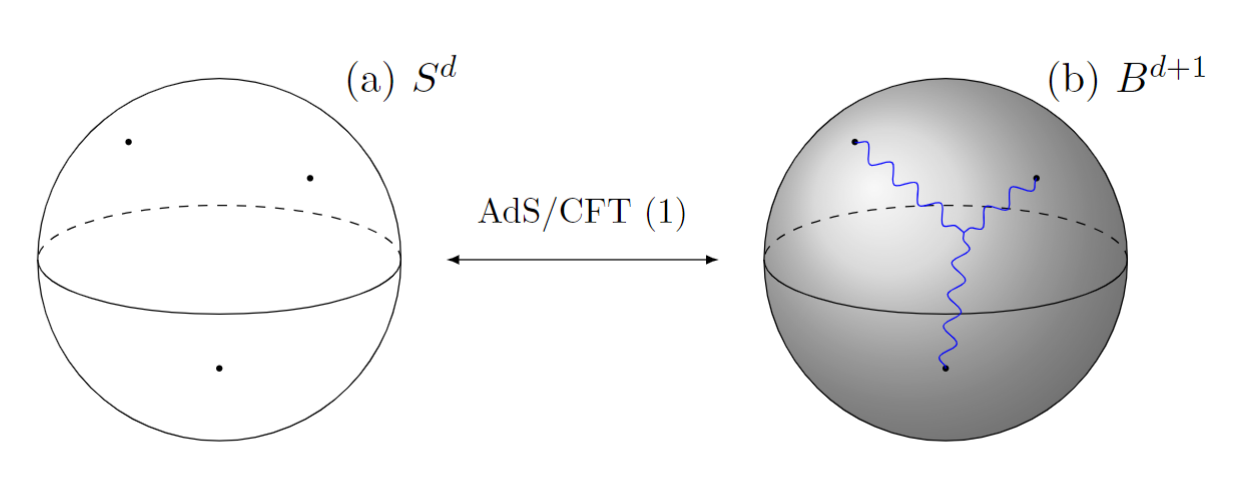
\includegraphics[scale=0.35]{Figures/ads cft.png}
\end{figure}

\item The original idea comes from consideration of the black hole entropy formula,
\eq{S_{BH}=\frac{\zt{Area}(\zt{Horizon})}{4G_N\hb}.}
It tells us that the black hole degrees of freedom live on the horizon, instead of in the interior.

\item Concrete examples are constructed from string theory.

\end{itemize}
\end{frame}


\begin{frame}{Internship - M1}
\begin{itemize}

\item 
Our case: holographic interface in AdS$_3$/CFT$_2$, a non-equilibrium steady state.
The interface in CFT corresponds to a thin brane (domain wall) in gravity.

\item
The model is exactly solvable and provides an example of a non-Killing horizon

% \item There is one rotating BTZ black hole on each side of the brane.

% \item We solve the shape of the brane using the Israel-Lanczos matching condition.

\begin{figure}[htb]
    \centering
    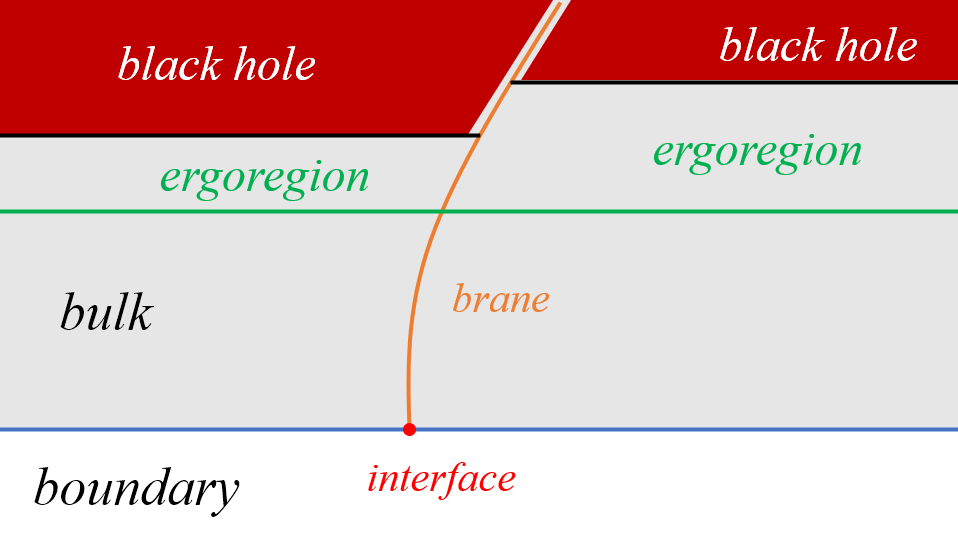
\includegraphics[scale=0.4]{Figures/btz.png}
\end{figure}

\end{itemize}
\end{frame}

\begin{frame}{Internship - M2}
\begin{itemize}

\item Quantum information. The entanglement entropy quantifies the amount of entanglement between two subregions in a QFT.
It is a difficult object to compute.

\item For holographic theories, the Ryu-Takayanagi formula tells us how to compute the entanglement entropy from bulk geometry,
\eq{S(\r_A)=\frac{\zt{Area}(\g)}{4G_N\hb}.}

\item The quantum information structure of the boundary theory can be mapped to the geometry in the bulk theory, and vice versa.
However, there are lots to understand in this perspective.

\begin{figure}[htb]
    \centering
    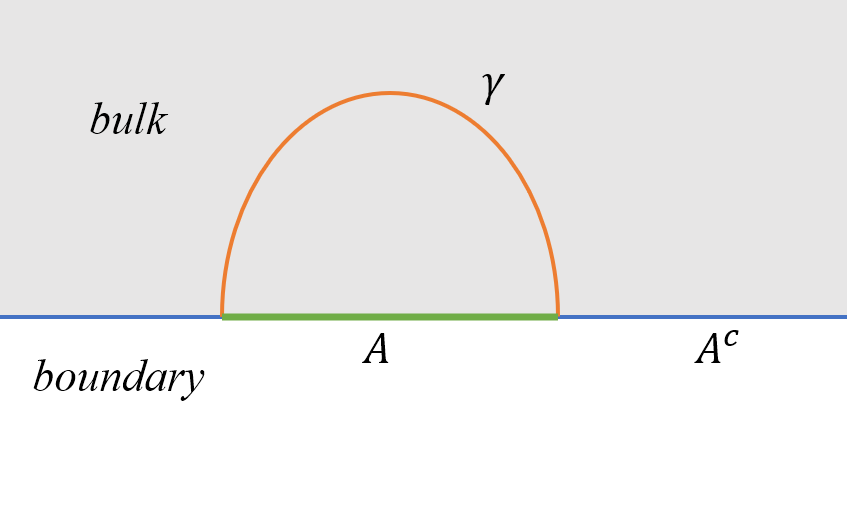
\includegraphics[scale=0.4]{Figures/RT formula.png}
\end{figure}

\end{itemize}
\end{frame}

\begin{frame}{Internship - M2}
\begin{itemize}

\item Tensor network: discretization of a spacial slice of the bulk spacetime, at least for the vacuum state.
Minimal cut $\iff$ RT surface.

\item Can we generalize this to interface CFT?
(Czech et al.)

\item How the relation between entropy and energy is reflected in the tensor network structure?

\begin{figure}[htb]
    \centering
    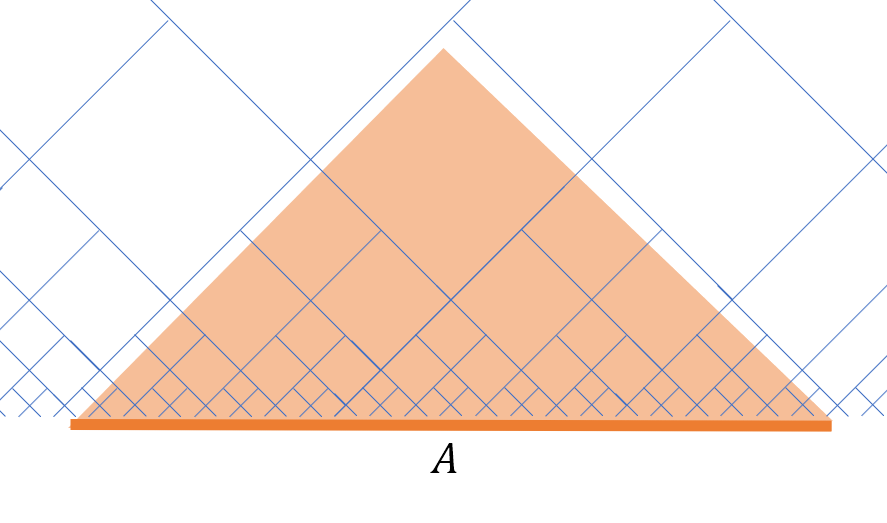
\includegraphics[scale=0.4]{Figures/mera network.png}
\end{figure}

\item Another task of the internship is to read the Snowmass white paper (2203.07117) of QI in QFT and QG, which is a review on the state of the subject.

\end{itemize}
\end{frame}

\begin{frame}{Thesis}
\begin{itemize}

\item We continue to study the solvable toy model of holographic interfaces, and use it to understand the relation between quantum information and geometry better.

\item This model is related to the recent island proposal, which is a possible solution to the black hole information paradox.

\item By examining the reconstruction of the island regions behind the horizon, we try to explain how unitarity is preserved in black hole evaporation.

\item At the end of the day, we would also like to understand the domain wall models constructed from string theory, different from our thin wall toy model.

\end{itemize}
\end{frame}


\begin{frame}{Thesis}
\begin{itemize}

Thank you for your attention!

\end{itemize}
\end{frame}




\end{document}